\documentclass[10pt,compress]{beamer}
\usetheme[hideothersubsections]{Berkeley}
\definecolor{aggiemaroon}{RGB}{80,0,0}
\usecolortheme[named=aggiemaroon]{structure}
\useoutertheme{shadow}
\useinnertheme{rounded}
\setbeamertemplate{navigation symbols}{}
\setbeamertemplate{mini frames}{}
\setbeamertemplate{headline}{}
\setbeamerfont{structure}{family=\rmfamily,series=\bfseries}
\usefonttheme[stillsansseriftext]{serif}

\usepackage{amsmath,amssymb,bm}
\usepackage{graphicx}
\usepackage{tikz}
\usetikzlibrary{positioning,arrows.meta,calc}
\usepackage{multicol}
\usepackage{hyperref}
\usepackage{booktabs}
\usepackage{array}
\usepackage{mathtools}

\newcommand{\R}{\mathbb{R}}
\newcommand{\E}{\mathbb{E}}
\newcommand{\prob}{\mathbb{P}}
\newcommand{\norm}[1]{\lVert #1\rVert}
\newcommand{\x}{\bm{x}}
\newcommand{\w}{\bm{w}}
\newcommand{\phiX}{\bm{\phi}}
\newcommand{\defline}[1]{{\footnotesize\textcolor{aggiemaroon}{\textit{#1}}\par}}

\title[Optimal-margin classifiers (1992)]{A Training Algorithm for Optimal Margin Classifiers}
\subtitle{A plain-language walkthrough of Boser, Guyon, and Vapnik (1992)}
\author[Thomas]{Nathaniel Thomas}
\date[October 19, 2026]{October 19, 2026}
\institute[Texas A\&M University]{Texas A\&M University}

\begin{document}
\begin{frame}\titlepage\end{frame}

% ------------------------------------------------------------------
\section[Motivation]{The problem and main idea}
\begin{frame}{1. Why does the margin matter?}
A classifier takes an input (for example, a digit image) and predicts one of two classes. A decision boundary divides the input space into the two predicted regions.
\begin{columns}[T]
\column{0.53\textwidth}
\begin{center}
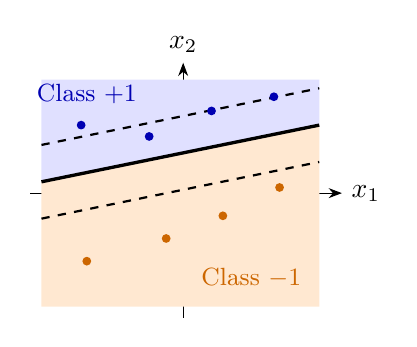
\begin{tikzpicture}[scale=0.72,>=Stealth]
\draw[->] (-2.7,0)--(2.8,0) node[right] {$x_1$};
\draw[->] (0,-2.2)--(0,2.3) node[above] {$x_2$};
\fill[blue!12] (-2.5,0.2) -- (-2.5,2) -- (2.4,2) -- (2.4,1.2) -- cycle;
\fill[orange!18] (-2.5,-2) -- (2.4,-2) -- (2.4,1.2) -- (-2.5,0.2) -- cycle;
\draw[very thick] (-2.5,0.2)--(2.4,1.2);
\draw[dashed,thick] (-2.5,-0.45)--(2.4,0.55);
\draw[dashed,thick] (-2.5,0.85)--(2.4,1.85);
\foreach \a/\b in {-1.8/1.2,-0.6/1.0,0.5/1.45,1.6/1.7}
  \fill[blue!70!black] (\a,\b) circle (2.2pt);
\foreach \a/\b in {-1.7/-1.2,-0.3/-0.8,0.7/-0.4,1.7/0.1}
  \fill[orange!80!black] (\a,\b) circle (2.2pt);
\node[blue!70!black] at (-1.7,1.75) {\small Class $+1$};
\node[orange!80!black] at (1.2,-1.5) {\small Class $-1$};
\end{tikzpicture}
\end{center}
\column{0.44\textwidth}
\begin{itemize}\small
\item Many boundaries may classify all training examples correctly.
\item A boundary that passes close to examples is fragile: small measurement or numerical changes can flip predictions.
\item The \textbf{margin} is the distance from the boundary to the nearest training examples.
\end{itemize}
\end{columns}
\defline{The paper's proposal: choose the separating rule with the largest possible margin, rather than merely one that fits the training set.}
{\scriptsize Boser, Guyon \& Vapnik (1992), Sec.~1.}
\end{frame}

\begin{frame}{2. The paper's setup: labels and a decision score}
Training data consist of $p$ labeled examples:
\[
(\x_1,y_1),\ldots,(\x_p,y_p), \qquad y_k\in\{-1,+1\}.
\]
The classifier computes a real-valued score $D(\x)$:
\[
\widehat y =
\begin{cases}
+1,&D(\x)>0,\\
-1,&D(\x)\leq 0.
\end{cases}
\]
A general form used by the paper is
\[
D(\x)=\w^\top\phiX(\x)+b.
\]
\defline{$\phiX(\x)$ transforms an input into features; $\w$ weights those features; $b$ shifts the boundary. The score's sign gives the class, while its magnitude indicates which side and how strongly.}
\begin{itemize}\small
\item The rule is linear in its adjustable parameters $\w,b$.
\item It need not be linear in the original input: the feature map can include products, nonlinear functions, or other transformations.
\end{itemize}
{\scriptsize Sec.~2, Eqs.~(1)--(7).}
\end{frame}

% ------------------------------------------------------------------
\section[Optimization]{How maximum margin becomes an optimization problem}
\begin{frame}{3. From geometric margin to a concrete objective}\footnotesize
For a correctly classified example, $y_kD(\x_k)>0$. Its signed geometric distance from the boundary is
\[
\frac{y_kD(\x_k)}{\norm{\w}}.
\]
The margin is the smallest such distance across all training examples:
\[
M=\min_{k=1,\ldots,p}\frac{y_kD(\x_k)}{\norm{\w}}.
\]
Rescaling $\w$ and $b$ changes score magnitudes but not the boundary, so the authors fix the scale by requiring $y_kD(\x_k)\geq 1$. Then maximizing the margin is equivalent to solving
\[
\boxed{\min_{\w,b}\;\frac12\norm{\w}^{2}
\quad\text{subject to}\quad
y_k(\w^\top\phiX(\x_k)+b)\geq 1.}
\]
\defline{The factor $1/2$ is mathematical convenience. Minimizing $\norm{\w}$ makes the margin $M^*=1/\norm{\w^*}$ as large as possible.}
\begin{block}{Intuition}
\small The classifier is not asked only to get every training label right; it is asked to do so with the largest buffer zone it can achieve.
\end{block}
{\scriptsize Sec.~2.1, Eqs.~(8)--(13).}
\end{frame}

\begin{frame}{4. Why use the dual problem?}
Directly optimizing $\w$ can be expensive when the feature space has a huge number of dimensions—or infinitely many. The authors use Lagrange multipliers $\alpha_k\geq0$ to turn the problem into one involving training examples and their pairwise similarities.
\[
\max_{\boldsymbol{\alpha}}\quad
\sum_{k=1}^{p}\alpha_k
-\frac12\sum_{k=1}^{p}\sum_{\ell=1}^{p}
\alpha_k\alpha_\ell y_ky_\ell
K(\x_k,\x_\ell)
\]
subject to
\[
\alpha_k\geq0,\qquad \sum_{k=1}^{p}\alpha_k y_k=0.
\]
Here $K(\x_k,\x_\ell)=\phiX(\x_k)^\top\phiX(\x_\ell)$ is a kernel: a similarity calculation that acts as an inner product in feature space.
\defline{The dual formulation lets the algorithm work with similarities between examples rather than explicitly building every transformed feature. The paper describes solving this constrained quadratic optimization numerically.}
{\scriptsize Sec.~2.2, Eqs.~(14)--(18); notation rewritten for readability.}
\end{frame}

\begin{frame}{5. Kernels: nonlinear boundaries without explicit features}
A kernel lets a linear separator in feature space correspond to a nonlinear boundary in the original input space.
\begin{columns}[T]
\column{0.52\textwidth}
\textbf{Polynomial kernel}
\[
K(\x,\x')=(\x^\top\x'+1)^q
\]
\small
The degree $q$ controls the interactions available to the classifier. For example, degree two includes pairwise products of input components.
\vspace{2mm}

\textbf{Radial-basis kernel}
\[
K(\x,\x')=\exp(-\gamma\norm{\x-\x'}^2)
\]
\small
Similarity is high for nearby points and falls as points move apart.
\column{0.43\textwidth}
\begin{center}
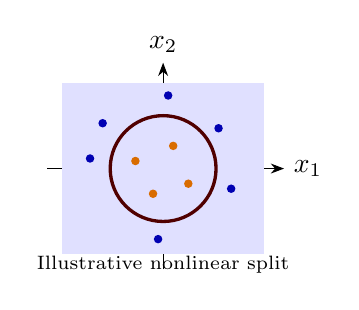
\begin{tikzpicture}[scale=0.64,>=Stealth]
\draw[->] (-2.3,0)--(2.4,0) node[right] {$x_1$};
\draw[->] (0,-2.0)--(0,2.1) node[above] {$x_2$};
\fill[blue!12] (-2,-1.7) rectangle (2,1.7);
\draw[very thick,aggiemaroon] (0,0) circle (1.05);
\foreach \a/\b in {-1.45/0.2,-1.2/0.9,1.35/-0.4,1.1/0.8,0.1/1.45,-0.1/-1.4}
\fill[blue!70!black] (\a,\b) circle (2.4pt);
\foreach \a/\b in {-0.55/0.15,0.5/-0.3,0.2/0.45,-0.2/-0.5}
\fill[orange!85!black] (\a,\b) circle (2.4pt);
\node at (0,-1.9) {\scriptsize Illustrative nonlinear split};
\end{tikzpicture}
\end{center}
\end{columns}
\defline{The paper discusses polynomial, radial-basis, and neural-network-related kernels. The RBF equation above uses a common modern parameterization; the paper's experiment uses $K(\x,\x')=\exp(-\norm{\x-\x'}/2)$.}
{\scriptsize Secs.~2 and 4, Eqs.~(5), (21), and Fig.~4.}
\end{frame}

% ------------------------------------------------------------------
\section[Support vectors]{What the solution depends on}
\begin{frame}{6. Support vectors: only the critical examples determine the boundary}\footnotesize
At the optimum, the weight vector can be written as
\[
\w^*=\sum_{k=1}^{p}\alpha_k y_k\phiX(\x_k),
\]
so the decision score becomes
\[
D(\x)=\sum_{k=1}^{p}\alpha_k y_k K(\x_k,\x)+b.
\]
The key condition is:
\[
\alpha_k>0 \quad\Longrightarrow\quad y_kD(\x_k)=1
\]
for the hard-margin solution. Examples with nonzero $\alpha_k$ are the \textbf{support vectors}.
\begin{columns}[T]
\column{0.5\textwidth}
\begin{itemize}\small
\item They lie on the margin boundary.
\item They anchor the learned separator.
\item Most other examples have $\alpha_k=0$ and do not appear in the final sum.
\end{itemize}
\column{0.46\textwidth}
\begin{center}
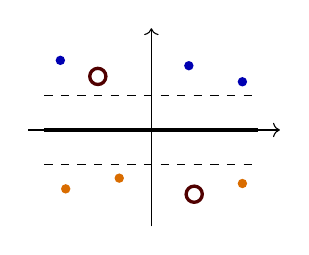
\begin{tikzpicture}[scale=0.68]
\draw[->] (-2.3,0)--(2.4,0);
\draw[->] (0,-1.8)--(0,1.9);
\draw[very thick] (-2.0,0)--(2.0,0);
\draw[dashed] (-2.0,0.65)--(2.0,0.65);
\draw[dashed] (-2.0,-0.65)--(2.0,-0.65);
\foreach \a/\b in {-1.7/1.3,-1.0/1.0,0.7/1.2,1.7/0.9}
\fill[blue!70!black] (\a,\b) circle (2.5pt);
\foreach \a/\b in {-1.6/-1.1,-0.6/-0.9,0.8/-1.2,1.7/-1.0}
\fill[orange!85!black] (\a,\b) circle (2.5pt);
\filldraw[white,draw=aggiemaroon,line width=1.2pt] (-1.0,1.0) circle (4.3pt);
\filldraw[white,draw=aggiemaroon,line width=1.2pt] (0.8,-1.2) circle (4.3pt);
\end{tikzpicture}
\end{center}
\end{columns}
\defline{This is the paper's central representation: the learned rule is a weighted combination of kernel functions centered on a subset of training examples.}
{\scriptsize Sec.~2.2, Eq.~(16) and following discussion.}
\end{frame}

\begin{frame}{7. Generalization, capacity, and atypical examples}\footnotesize
The authors argue that a large margin helps the classifier generalize: it avoids choosing an unnecessarily fragile separator among those that fit the training set.
\begin{itemize}\small
\item \textbf{Capacity tuning:} the kernel controls the family of possible boundaries, while maximum-margin training selects a separator within that family.
\item \textbf{Leave-one-out bound:} removing a non-support vector leaves the boundary unchanged. The paper derives an error bound related to the number of linearly independent support vectors divided by the number of training examples.
\item \textbf{Outlier identification:} examples with large $\alpha_k$ strongly influence the boundary and can flag atypical or ambiguous records for review.
\end{itemize}
\begin{block}{Important distinction}
\small A large margin is a principled objective, not a guarantee that every dataset will generalize well. The paper's bounds and conclusions depend on the setup and assumptions.
\end{block}
\defline{The 1992 paper is a hard-margin formulation for separable data, with discussion of removing atypical patterns; it is not the later soft-margin SVM formulation with a regularization parameter $C$.}
{\scriptsize Secs.~1 and 3.1, especially the leave-one-out discussion on pp.~147--148.}
\end{frame}

% ------------------------------------------------------------------
\section[Experiments]{Experiments and findings}
\begin{frame}{8. Experiment: handwritten digit recognition}
The authors evaluate on two handwritten-digit image datasets. Each image is $16\times16$ pixels, so an image can be represented by 256 input values. They train ten decision surfaces, one for each digit class.
\begin{table}
\centering\scriptsize
\begin{tabular}{>{\raggedright\arraybackslash}p{1.3cm}
                >{\raggedright\arraybackslash}p{1.7cm}
                >{\raggedright\arraybackslash}p{1.7cm}
                >{\raggedright\arraybackslash}p{3.6cm}}
\toprule
Dataset & Training & Test & Description \\
\midrule
DB1 & 600 images & 600 images & Clean images from 10 subjects \\
DB2 & 7,300 images & 2,000 images & Images from actual mail pieces; includes ambiguous or meaningless patterns \\
\bottomrule
\end{tabular}
\end{table}
\begin{itemize}\tiny
\item DB1 tests generalization on a relatively clean dataset.
\item DB2 tests a larger, messier real-world dataset.
\item The paper compares linear and nonlinear kernels, and also investigates smoothing as preprocessing.
\end{itemize}
\defline{The paper reports using the same preprocessing and similarity function across the ten class surfaces in each experiment.}
{\scriptsize Sec.~4, pp.~149--150.}
\end{frame}

\begin{frame}{9. Results: nonlinear features help, and data quality matters}\footnotesize
\begin{columns}[T]
\column{0.49\textwidth}
\textbf{Clean DB1}
\begin{itemize}\small
\item Linear maximum-margin classifier: zero training error, 3.2\% test error.
\item Linear MSE-based comparison: 12.7\% test error.
\item A second-order polynomial with smoothing achieved 0.3\% test error in the reported table.
\end{itemize}
\column{0.49\textwidth}
\textbf{Mail-image DB2}
\begin{itemize}\small
\item Linear classifier: 15.2\% test error before cleaning.
\item Removing selected ambiguous/meaningless patterns reduced error to 10.5\%.
\item A fourth-order polynomial reached 4.9\% test error; a fifth-order neural network result cited by the paper was 5.1\%.
\end{itemize}
\end{columns}
\begin{center}
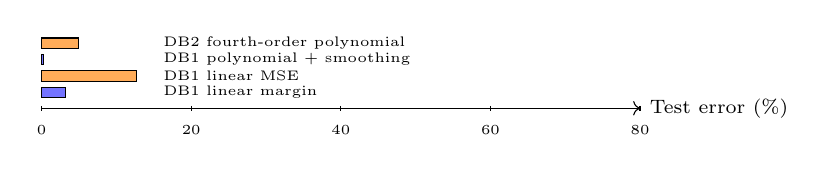
\begin{tikzpicture}[x=0.095cm,y=0.38cm]
\draw[->] (0,0)--(80,0) node[right] {\scriptsize Test error (\%)};
\foreach \xv in {0,20,40,60,80} {\draw (\xv,0.08)--(\xv,-0.08) node[below=2pt] {\tiny \xv};}
\draw[fill=blue!55] (0,0.35) rectangle (3.2,0.7);
\draw[fill=orange!65] (0,0.9) rectangle (12.7,1.25);
\draw[fill=blue!55] (0,1.45) rectangle (0.3,1.8);
\draw[fill=orange!65] (0,2.0) rectangle (4.9,2.35);
\node[anchor=west] at (15,0.53) {\tiny DB1 linear margin};
\node[anchor=west] at (15,1.08) {\tiny DB1 linear MSE};
\node[anchor=west] at (15,1.63) {\tiny DB1 polynomial + smoothing};
\node[anchor=west] at (15,2.18) {\tiny DB2 fourth-order polynomial};
\end{tikzpicture}
\end{center}
\defline{Reported values are from the paper; the smoothing result is DB1 with Gaussian smoothing parameter $\sigma=1.0$. The paper's results are specific to these datasets and experimental setup.}
{\scriptsize Sec.~4, pp.~149--150.}
\end{frame}

\begin{frame}{10. What the paper contributes—and what it does not}\scriptsize
\begin{columns}[T]
\column{0.49\textwidth}
\textbf{Contributions}
\begin{itemize}\scriptsize
\item A maximum-margin training objective.
\item A dual, kernel-based representation that avoids explicit high-dimensional features.
\item A sparse solution depending on support vectors.
\item A theoretical discussion of generalization and outlier detection.
\item Early experimental evidence on handwritten-digit recognition.
\end{itemize}
\column{0.49\textwidth}
\textbf{Scope and caveats}
\begin{itemize}\scriptsize
\item The main derivation assumes separable training data.
\item The paper's algorithm is not the later soft-margin formulation.
\item The number of support vectors and test error depend on kernel, preprocessing, and data quality.
\item A maximum margin does not remove the need for validation or good features.
\end{itemize}
\end{columns}
\begin{block}{Take-home message}
\small Rather than just finding a boundary that fits the examples, the method finds a wide-margin boundary and expresses it using only the examples that constrain it most strongly.
\end{block}

\end{frame}

\begin{frame}{References}
\footnotesize
\begin{thebibliography}{9}
\bibitem{boser92}
B. E. Boser, I. M. Guyon, and V. N. Vapnik.
\newblock A Training Algorithm for Optimal Margin Classifiers.
\newblock In \emph{Proceedings of the Fifth Annual Workshop on Computational Learning Theory (COLT '92)}, pp.~144--152, 1992.
\newblock DOI: \href{https://doi.org/10.1145/130385.130401}{10.1145/130385.130401}.
\bibitem{vapnik}
V. N. Vapnik.
\newblock \emph{Estimation of Dependences Based on Empirical Data}.
\newblock Springer, 1982.
\end{thebibliography}
\vfill
\small Presentation based primarily on the supplied paper. Explanatory diagrams are schematic and are not reproductions of the paper's figures.
\end{frame}

\end{document}
